\section{Proceso de creación de conjunto de datos}

El diagrama de flujo de la Figura \ref{fig:DFCreacionCD} muestra el proceso completo para generar un conjunto de datos, en este vemos que una vez que se toman todas las muestras los tres siguientes pasos son iterativos hasta que las hayamos procesado todas.

\begin{figure}[H]
    \centering
    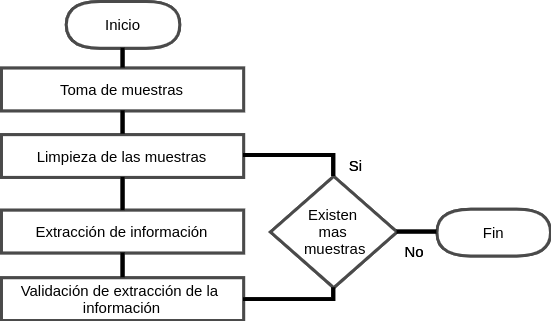
\includegraphics[width=0.9\textwidth]{Metodologia/imgs/FlowSystem.png}
    \caption{Diagrama de flujo para la creacion de conjunto de datos.}
    \label{fig:DFCreacionCD}
\end{figure}

%%%%%%%%%%%%%%%%%%%%%%%%%%%%%%%%%%%%%%%%%%%%%%%%%%%%%%%%%%%%%%%%%%%%%%%%%%%%%%%%
%%%%%%%%%%%%%%%%%%%%%%%%%%%%%%%%%%%%%%%%%%%%%%%%%%%%%%%%%%%%%%%%%%%%%%%%%%%%%%%%
%%%%%%%%%%%%%%%%%%%%%%%%%%%%%%%%%%%%%%%%%%%%%%%%%%%%%%%%%%%%%%%%%%%%%%%%%%%%%%%%
%%%%%%%%%%%%%%%%%%%%%%%%%%%%%%%%%%%%%%%%%%%%%%%%%%%%%%%%%%%%%%%%%%%%%%%%%%%%%%%%
%%%%%%%%%%%%%%%%%%%%%%%%%%%%%%%%%%%%%%%%%%%%%%%%%%%%%%%%%%%%%%%%%%%%%%%%%%%%%%%%

\subsection{Toma de muestras}

La primera etapa correspondió de Toma de Muestras, se requirió de dos dispositivos para la extracción de conjunto de datos que posteriormente se utilizara como entrenamiento de los modelos predictivos. Uno de los dispositivos es el radar Bushnell (Figura \ref{fig:RadarVelocidad}) con una precisión de +/- 1.6 kilómetros por hora.

\begin{figure}[H]
    \centering
    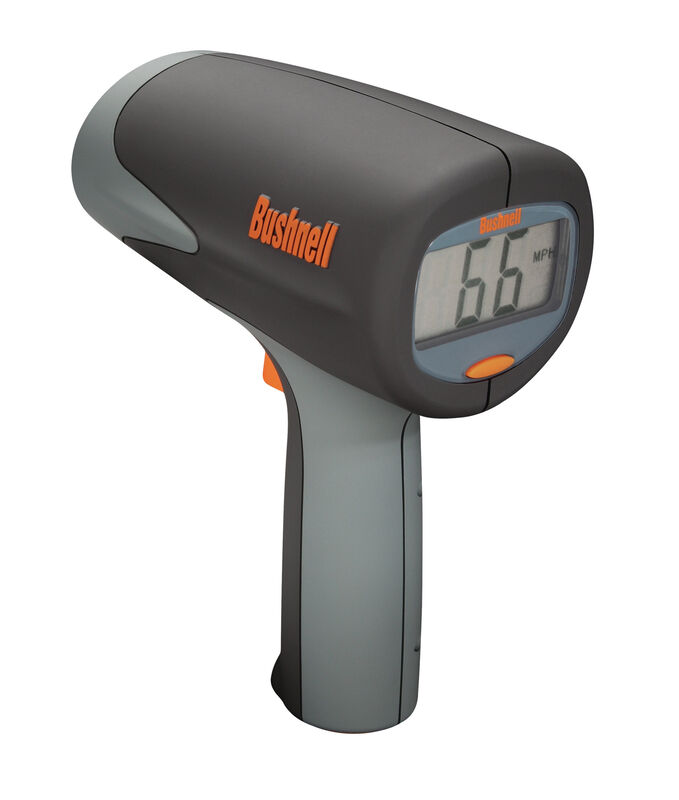
\includegraphics[width=0.4\textwidth]{Metodologia/imgs/bushnell.jpg}
    \caption{Radar de velocidad Bushnell.}
    \label{fig:RadarVelocidad}
\end{figure}

Mientras que el otro dispositivo es una cámara de video, la cual puede ser un dispositivo especializado para esta tarea o cualquier otro dispositivo capaz de grabar video. Las configuraciones mínimas pueden ser una resolución de 854 x 480 a 30 fotogramas por segundo, sin embargo, hay que tomar en cuenta que al tener una resolución tan baja podemos perder calidad en la imagen y tomar un área menor a la deseada, mientras que tener fotogramas tan bajos nos ocasionaría perder vehículo que pasan a una velocidad más alta. Por otro parte al aumentar la resolución y los fotogramas por segundo estamos ocasionando que al sistema le tome más tiempo procesarlos. Para este caso se utilizó la cámara de Smartphones un Xiaomi Redmi Note 7 y un iPhone X configurados a 60 FPS y una resolución de Full HD (1920 x 1080 pixeles).

Se tomo especial cuidado a la hora de posicionar la cámara, ya que no se quiere que los experimentos sean considerados como cálculos de velocidad en 2D, para esto la toma de muestras se realizó en un lugar donde el tráfico vehicular pase con cierto grado de inclinación, sin apuntar la cámara directamente al costado de donde pasan los vehículos, como muestra la Figura \ref{fig:LugarMuestras}.

\begin{figure}[H]
    \centering
    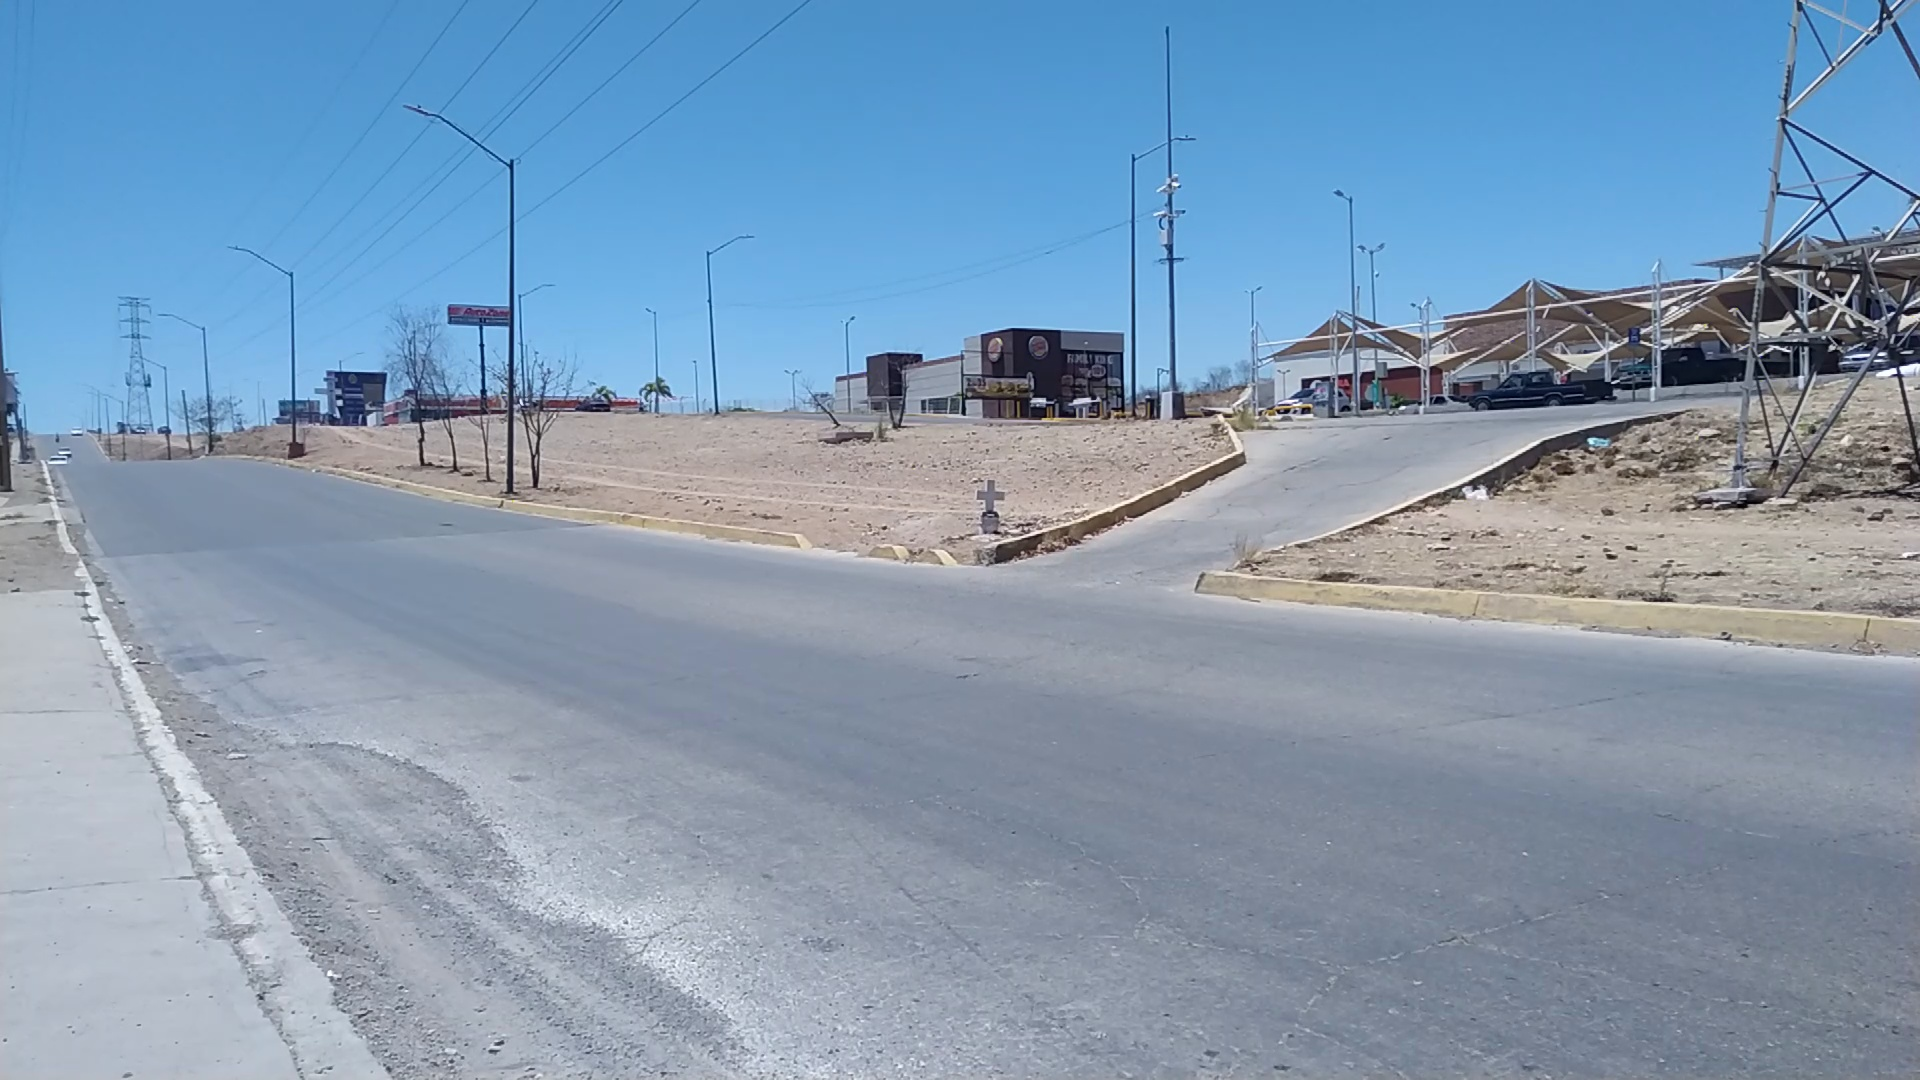
\includegraphics[width=0.8\textwidth]{Metodologia/imgs/LugarMuestras.jpg}
    \caption{Lugar donde se tomaron las muestras.}
    \label{fig:LugarMuestras}
\end{figure}

Cabe mencionar que para hacer más practica y rápido la toma de muestras, estas fueron tomadas en este mismo lugar, en la ciudad de Culiacán, Sinaloa.

Dado que la cámara y el radar de velocidad son dispositivos que no están sincronizados entre si para darnos el video y la velocidad, nos aseguramos se guardar la velocidad detectada por el radar en el video tomada, diciéndola en voz alta al micrófono de la cámara.

%%%%%%%%%%%%%%%%%%%%%%%%%%%%%%%%%%%%%%%%%%%%%%%%%%%%%%%%%%%%%%%%%%%%%%%%%%%%%%%%
%%%%%%%%%%%%%%%%%%%%%%%%%%%%%%%%%%%%%%%%%%%%%%%%%%%%%%%%%%%%%%%%%%%%%%%%%%%%%%%%
%%%%%%%%%%%%%%%%%%%%%%%%%%%%%%%%%%%%%%%%%%%%%%%%%%%%%%%%%%%%%%%%%%%%%%%%%%%%%%%%
%%%%%%%%%%%%%%%%%%%%%%%%%%%%%%%%%%%%%%%%%%%%%%%%%%%%%%%%%%%%%%%%%%%%%%%%%%%%%%%%
%%%%%%%%%%%%%%%%%%%%%%%%%%%%%%%%%%%%%%%%%%%%%%%%%%%%%%%%%%%%%%%%%%%%%%%%%%%%%%%%

\subsection{Limpieza de las muestras}

Una vez tomadas las muestras es necesario realizar una limpieza de los datos, estos son, los vehículos a los que se les tomo la velocidad utilizando el radar. Ya que el video y el radar no están sincronizados por hardware es necesario realizar una inspección visual de las muestras.

Considerando que la cámara de video y el radar no son dispositivos especializados para esta tarea, fue necesario encontrar una manera de unir los datos del video con la velocidad, así que se implementó el sistema pensando en que recibiría como entrada un archivo CSV con el mismo nombre que la muestra, pero con la extensión TXT. Este archivo contiene los datos necesarios para realizar la unión de las características del video y la velocidad, los valores del archivo son los siguientes:

\begin{itemize}
    \item Segundo en que pasa el vehículo
    \item Velocidad detectada por el radar
    \item Carril
    \item Descripción del vehículo
\end{itemize}

Para poder determinar la velocidad siempre es necesario tomar el tiempo que le toma a un objeto pasar de un lugar a otro, para esto el sistema necesita ser configurado con un punto de entrada y un punto de salida en el eje X, para fines prácticos a partir de ahora llamaremos a estos dos puntos simplemente punto A y punto B.  Estos dos puntos deben ser colocados de manera que los vehículos deben pasar completamente por cada uno de ellos, además que cada una de las muestras pueden tener diferentes valores para los puntos A y B, sin embargo, para nuestro caso no fue necesario implementar diferentes valores ya que todos los videos fueron tomados en el mismo lugar. La Figura \ref{fig:LugarLimites} muestras donde fueron colocados los puntos A y B en nuestras muestras.

\begin{figure}[H]
    \centering
    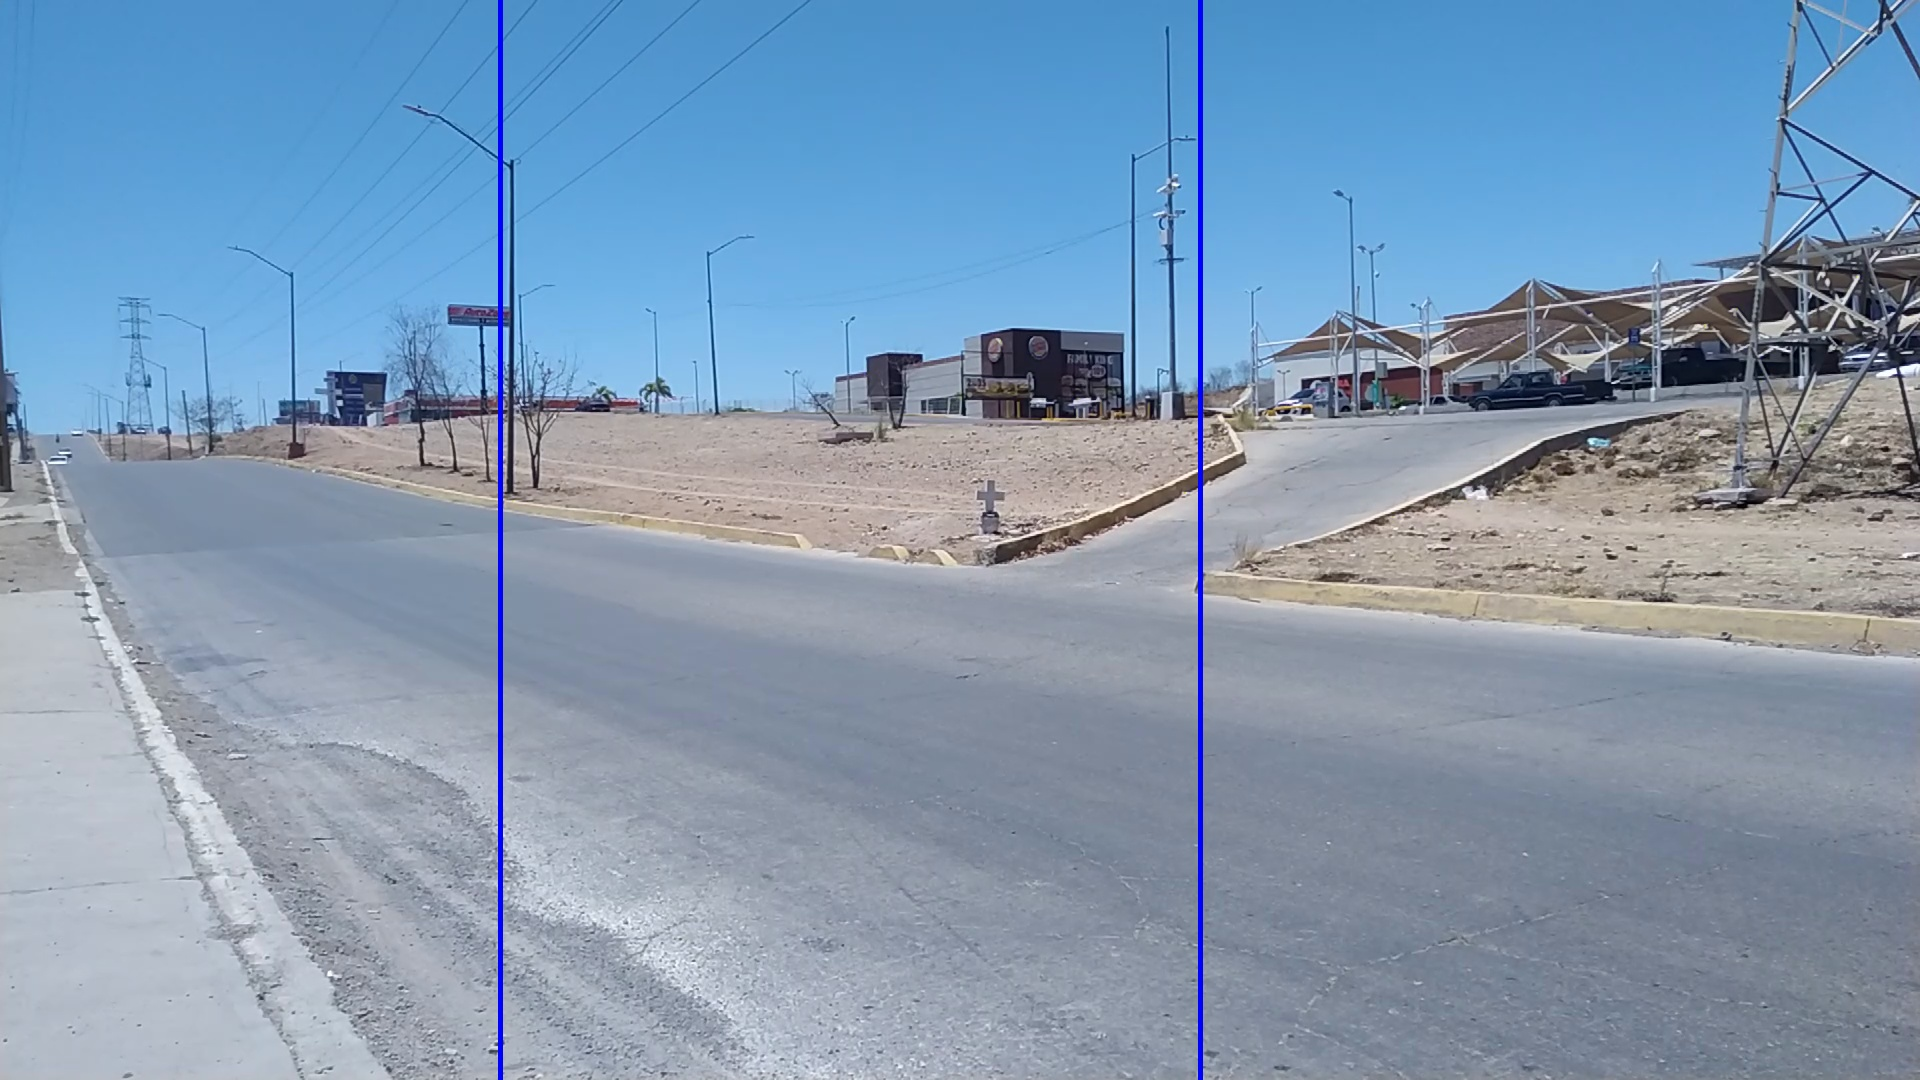
\includegraphics[width=0.8\textwidth]{Metodologia/imgs/LugarLimites.jpg}
    \caption{Limites para lugar de las muestras.}
    \label{fig:LugarLimites}
\end{figure}

Una vez que tenemos los valores para los puntos A y B podemos comenzar a generar el archivo CVS, para esto debemos tomar en cuenta que el segundo en que pasa debe ser lo más cercano posible al centro del vehículo cuando pasa por el punto B, es importante ingresar una descripción, aunque esta no va a ser usada por el sistema, se volverá importante para validar que el vehículo al que se le tomo la velocidad es el mismo que detecto el sistema.

%%%%%%%%%%%%%%%%%%%%%%%%%%%%%%%%%%%%%%%%%%%%%%%%%%%%%%%%%%%%%%%%%%%%%%%%%%%%%%%%
%%%%%%%%%%%%%%%%%%%%%%%%%%%%%%%%%%%%%%%%%%%%%%%%%%%%%%%%%%%%%%%%%%%%%%%%%%%%%%%%
%%%%%%%%%%%%%%%%%%%%%%%%%%%%%%%%%%%%%%%%%%%%%%%%%%%%%%%%%%%%%%%%%%%%%%%%%%%%%%%%
%%%%%%%%%%%%%%%%%%%%%%%%%%%%%%%%%%%%%%%%%%%%%%%%%%%%%%%%%%%%%%%%%%%%%%%%%%%%%%%%
%%%%%%%%%%%%%%%%%%%%%%%%%%%%%%%%%%%%%%%%%%%%%%%%%%%%%%%%%%%%%%%%%%%%%%%%%%%%%%%%

\subsection{Extracción de información }

Una vez que hemos tomado la muestra y generado el archivo CSV relacionado podemos ejecutar el sistema para extraer las características que nos interesa junto a la velocidad detectada por el radar de velocidad.

El sistema se encarga de leer el video utilizando la biblioteca OpenCV con la cual examina fotograma por fotograma, e identifica los vehículos utilizando la red neuronal YOLO, una vez que tiene identificados todos los vehículos dibuja la caja correspondiente a cada uno de ellos. La Figura \ref{fig:LugarDeteccion} muestra 2 vehículos detectados, los cuales están dentro de un recuadro.

\begin{figure}[H]
    \centering
    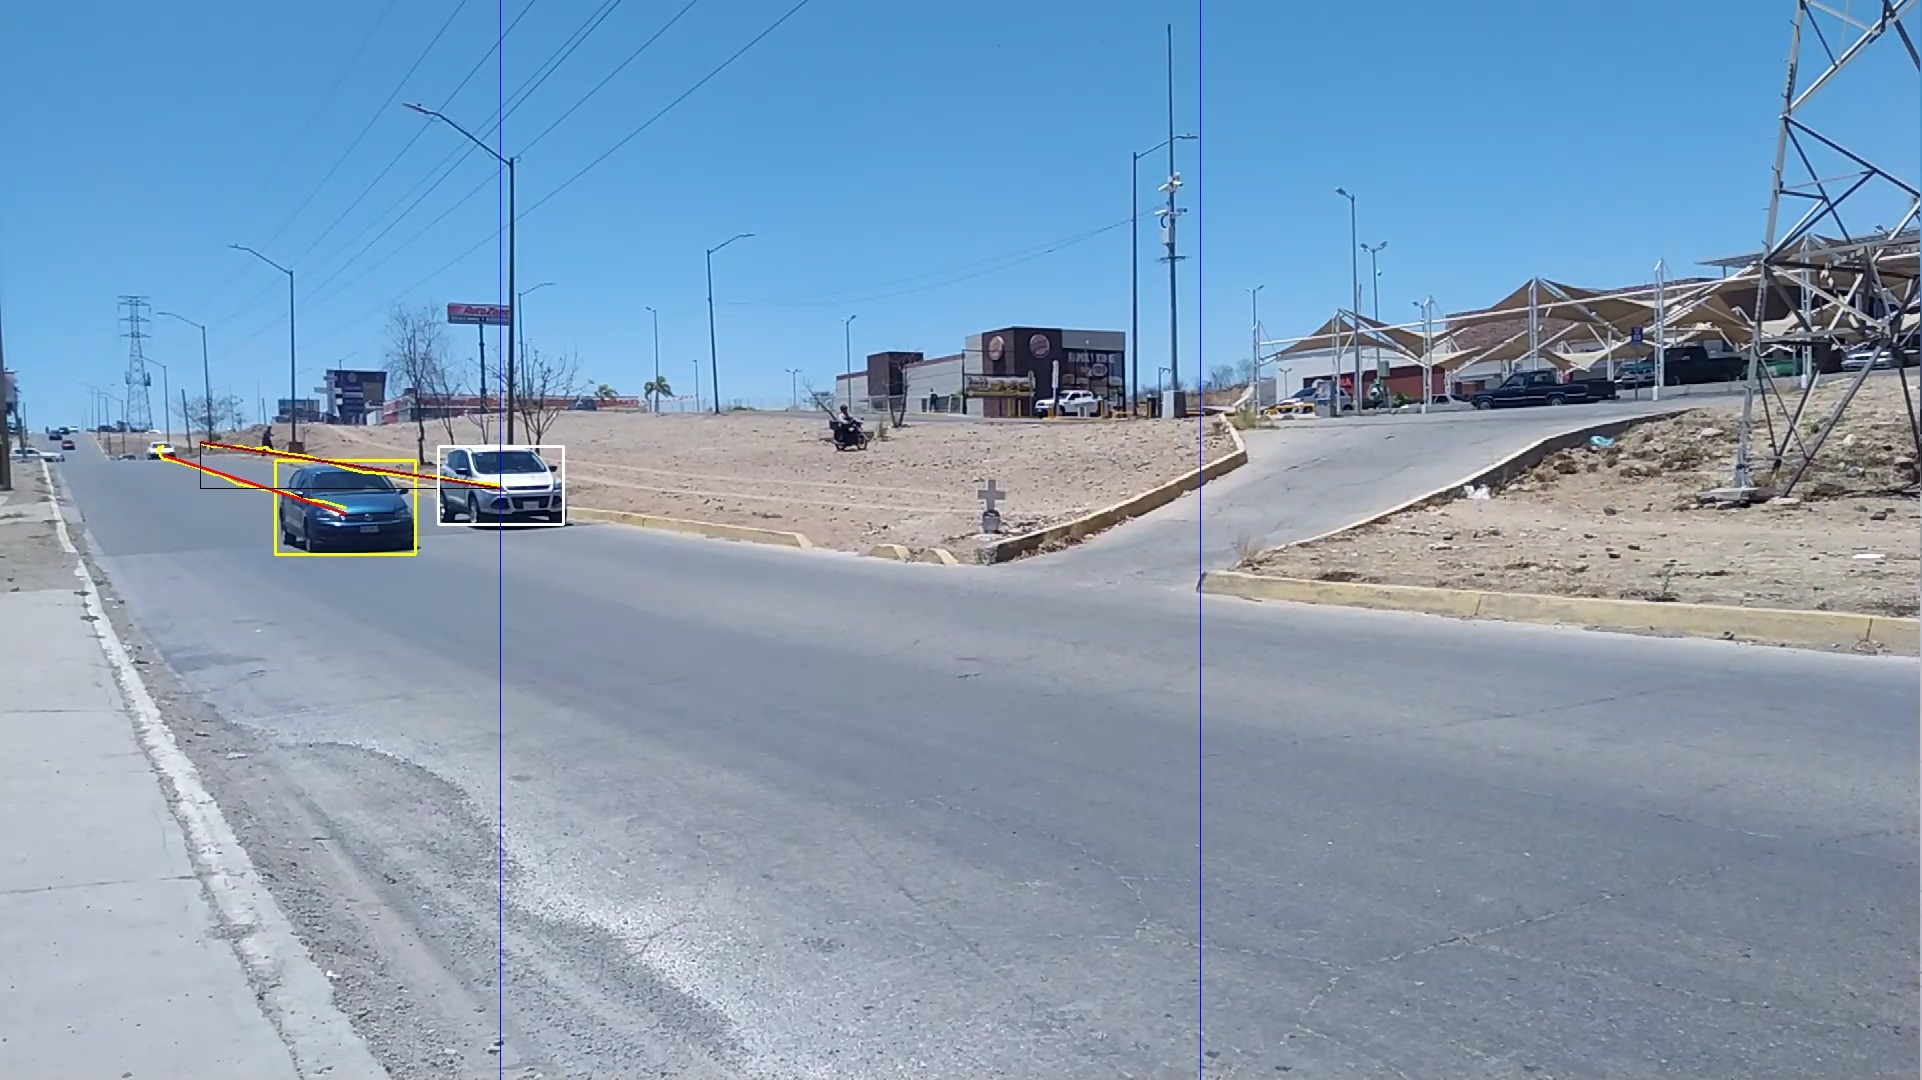
\includegraphics[width=0.8\textwidth]{Metodologia/imgs/Deteccion.jpg}
    \caption{Detección de vehículos dentro de recuadros.}
    \label{fig:LugarDeteccion}
\end{figure}

El seguimiento de los vehículos se realiza por medio del filtro Kalman para determinar su ubicación en el próximo fotograma. El sistema se encarga de guardar todas las ubicaciones de los vehículos en el transcurso del tiempo, con lo cual es capaz dibujar todo el trayecto que han tenido cada uno de ellos y con el uso de regresión lineal podemos generar una recta que corresponde a las trayectorias de los vehículos, la Figura \ref{fig:LugarSeguimiento} muestra un vehículo detectado en un recuadro blanco, así como un par de líneas una amarilla y otra roja que corresponden al seguimiento del mismo y a la recta calculada correspondiente al seguimiento.

\begin{figure}[H]
    \centering
    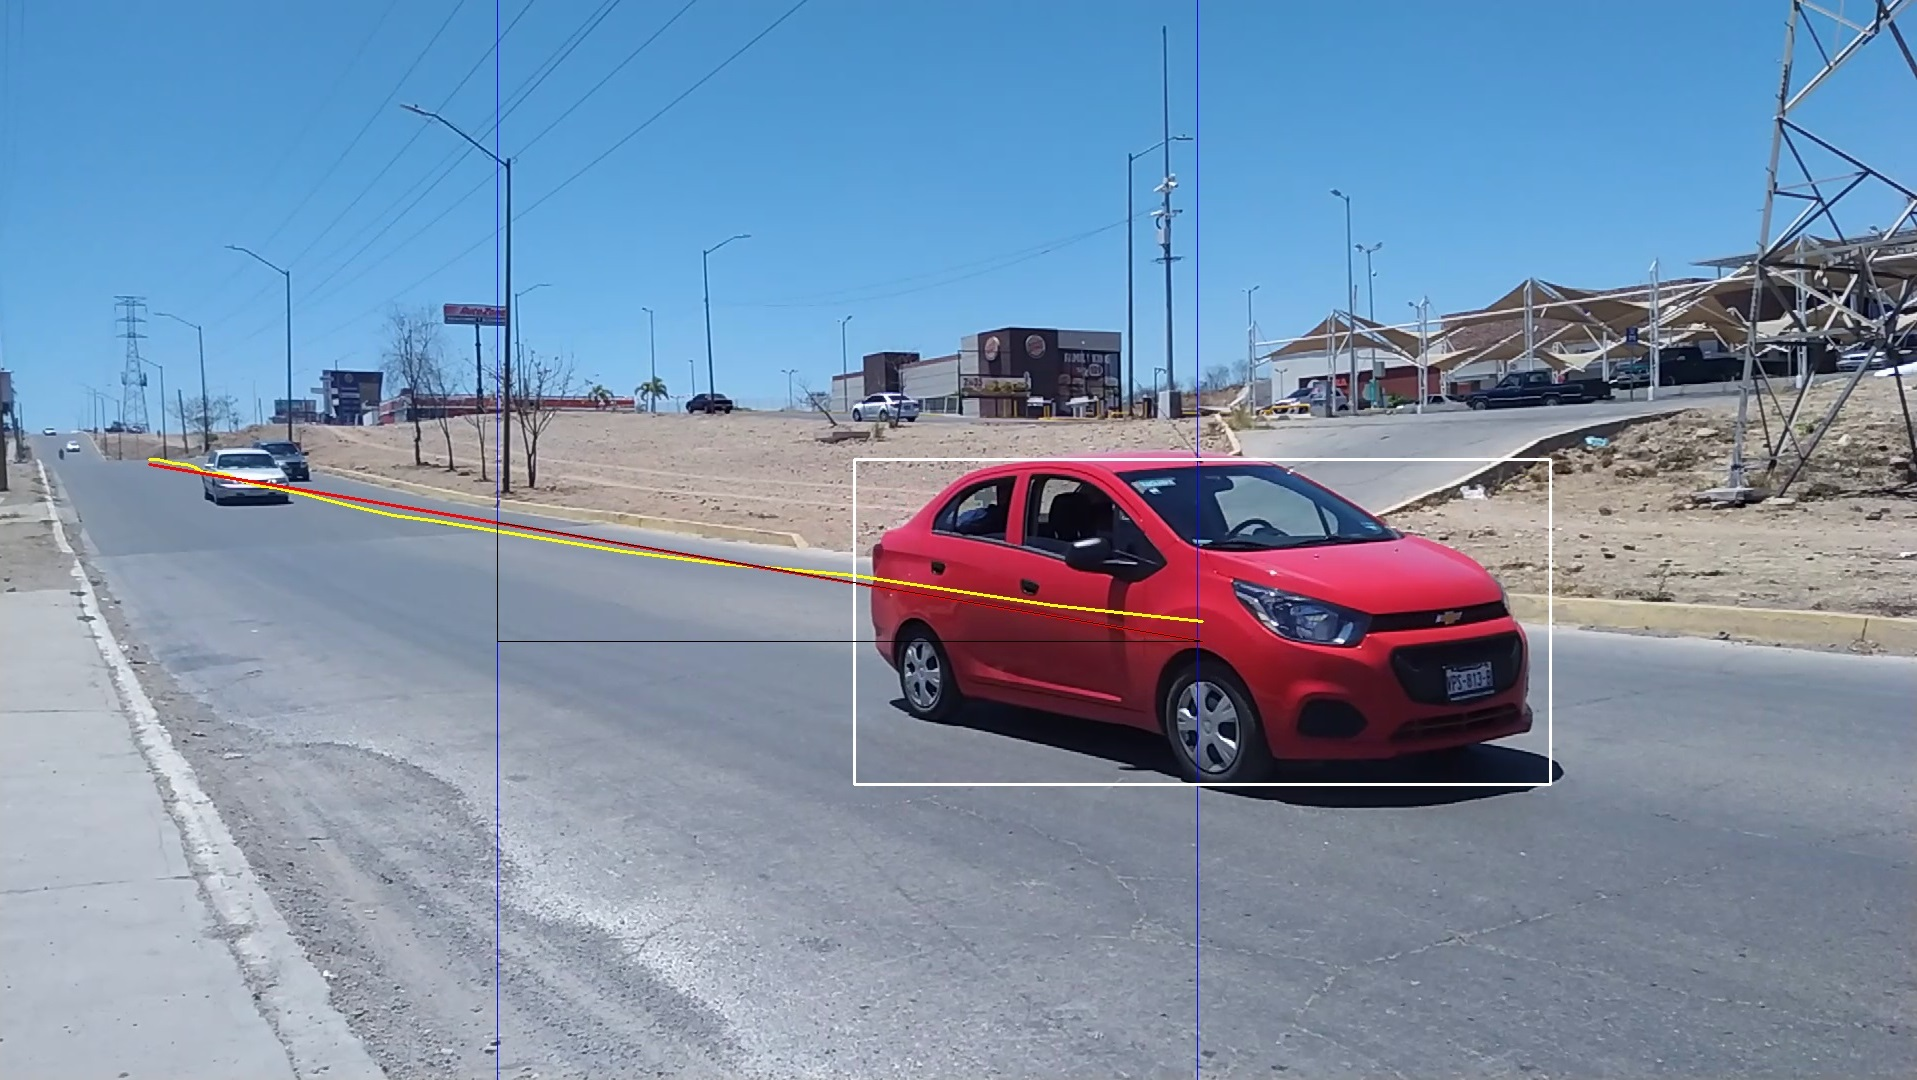
\includegraphics[width=0.8\textwidth]{Metodologia/imgs/Seguimiento.jpg}
    \caption{Detección de vehículos y sus trayectorias.}
    \label{fig:LugarSeguimiento}
\end{figure}

Otra característica que podemos identificar en la Figura \ref{fig:LugarSeguimiento} es la creación de un triángulo en color negro, con el cual podemos identificar el ángulo detectado para el vehículo.

Cando el sistema detecta que un vehículo pasa por el punto A, este guarda la información del estado del vehículo Figura \ref{fig:PuntoA}, puede haber múltiples vehículos pasando en ese momento y todos serán detectados por YOLO, sin embargo, podemos identificar el vehículo del cual se está guardando su estado con el recuadro blanco, ya que para el resto de vehículos se dibuja un recuadro amarillo.

\begin{figure}[H]
    \centering
    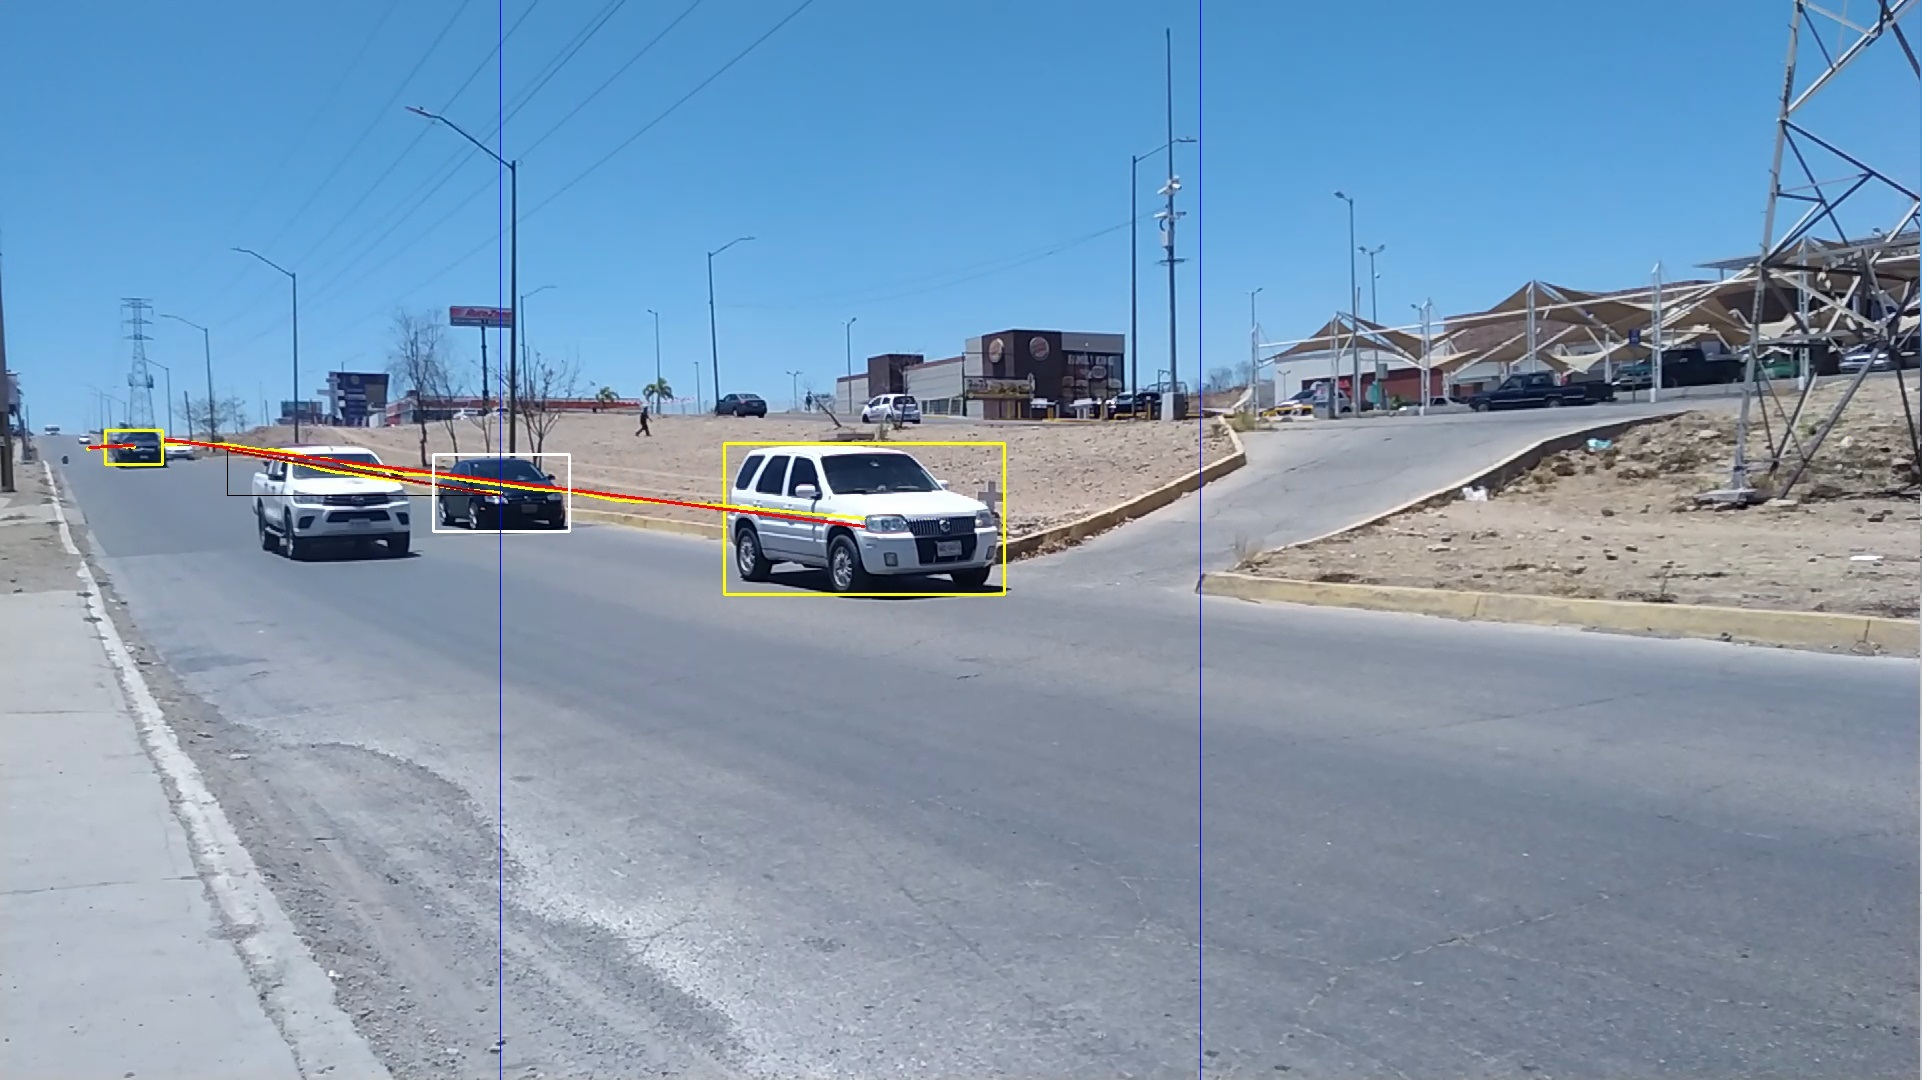
\includegraphics[width=0.8\textwidth]{Metodologia/imgs/Punto_A.jpg}
    \caption{Punto A con vehículo en recuadro blanco.}
    \label{fig:PuntoA}
\end{figure}

Aunque se guardó el estado del vehículo cuando paso por el punto A, este no genera una línea para el archivo CSV resultante, es hasta que el vehículo pasa por el punto B y coincide con los segundos en el archivo CSV de entrada que el sistema guarda un nuevo dato en el archivo de salida, los vehículos que no cuentan con una línea en el archivo CSV de entrada no se les guarda su información. La Figura \ref{fig:PuntoB} muestra cuando el vehículo detectado en el punto A pasa por el punto B.

\begin{figure}[H]
    \centering
    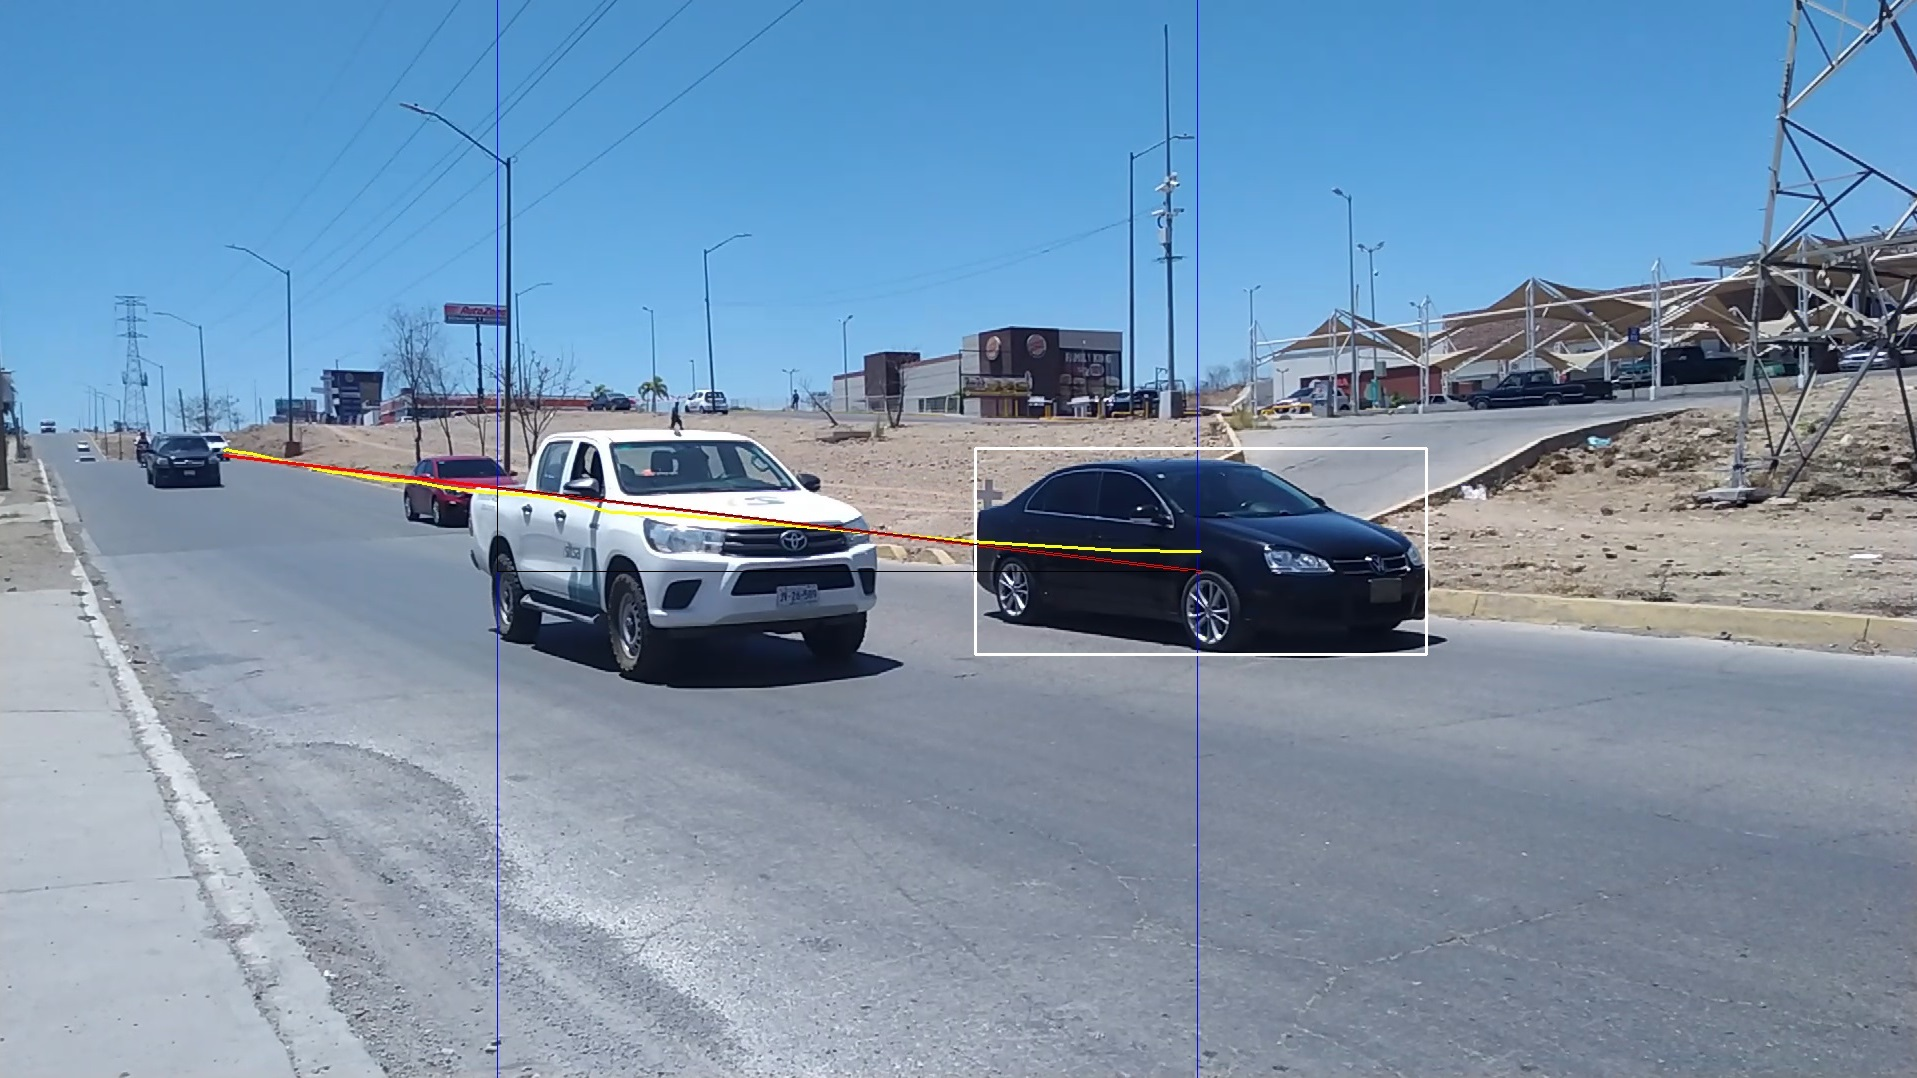
\includegraphics[width=0.8\textwidth]{Metodologia/imgs/Punto_B.jpg}
    \caption{Punto B con vehículo en recuadro blanco.}
    \label{fig:PuntoB}
\end{figure}

La Tabla \ref{tab:CaracteristicasSistema} muestra las características más importantes generadas por el sistema y su descripción.

\begin{table}[H]
    \caption{Características obtenidas por el sistema.}
    \label{tab:CaracteristicasSistema}
    \begin{tabular}{|l|l|}
        \hline
        \multicolumn{1}{|c|}{\textbf{Característica}} & \multicolumn{1}{c|}{\textbf{Descripción}}                                \\ \hline
        Angulo Salida                                 & Angulo a partir del punto de entrada hasta el punto de salida            \\ \hline
        Distancia de salida                           & Distancia recorrida desde el punto de entrada hasta el punto de salida   \\ \hline
        Área Entrada                                  & Área detectada del vehículo en pixeles en el punto de entrada            \\ \hline
        Área Salida                                   & Área detectada del vehículo en pixeles en el punto de salida             \\ \hline
        FPS                                           & Fotogramas por segundo del video                                         \\ \hline
        Tiempo                                        & Tiempo que le tomo al vehículo para pasar del punto entrada al de salida \\ \hline
        Velocidad                                     & Velocidad detectada por el radar                                         \\ \hline
        Carril                                        & Carril por que pasa el vehículo                                          \\ \hline
        Identificador                                 & Identificador correspondiente a una imagen generada                      \\ \hline
    \end{tabular}
\end{table}


El sistema además de generar un archivo CSV, nos da una imagen de salida la cual corresponde a una línea del archivo resultante, esta imagen está formada por dos imágenes una al lado de la otra, la imagen de la izquierda representa el vehículo cuando entra en el punto A y la imagen de la derecha es cuando el vehículo pasa por el punto B. La Figura IMAGEN muestra un ejemplo de esta imagen de salida.

\begin{figure}[H]
    \centering
    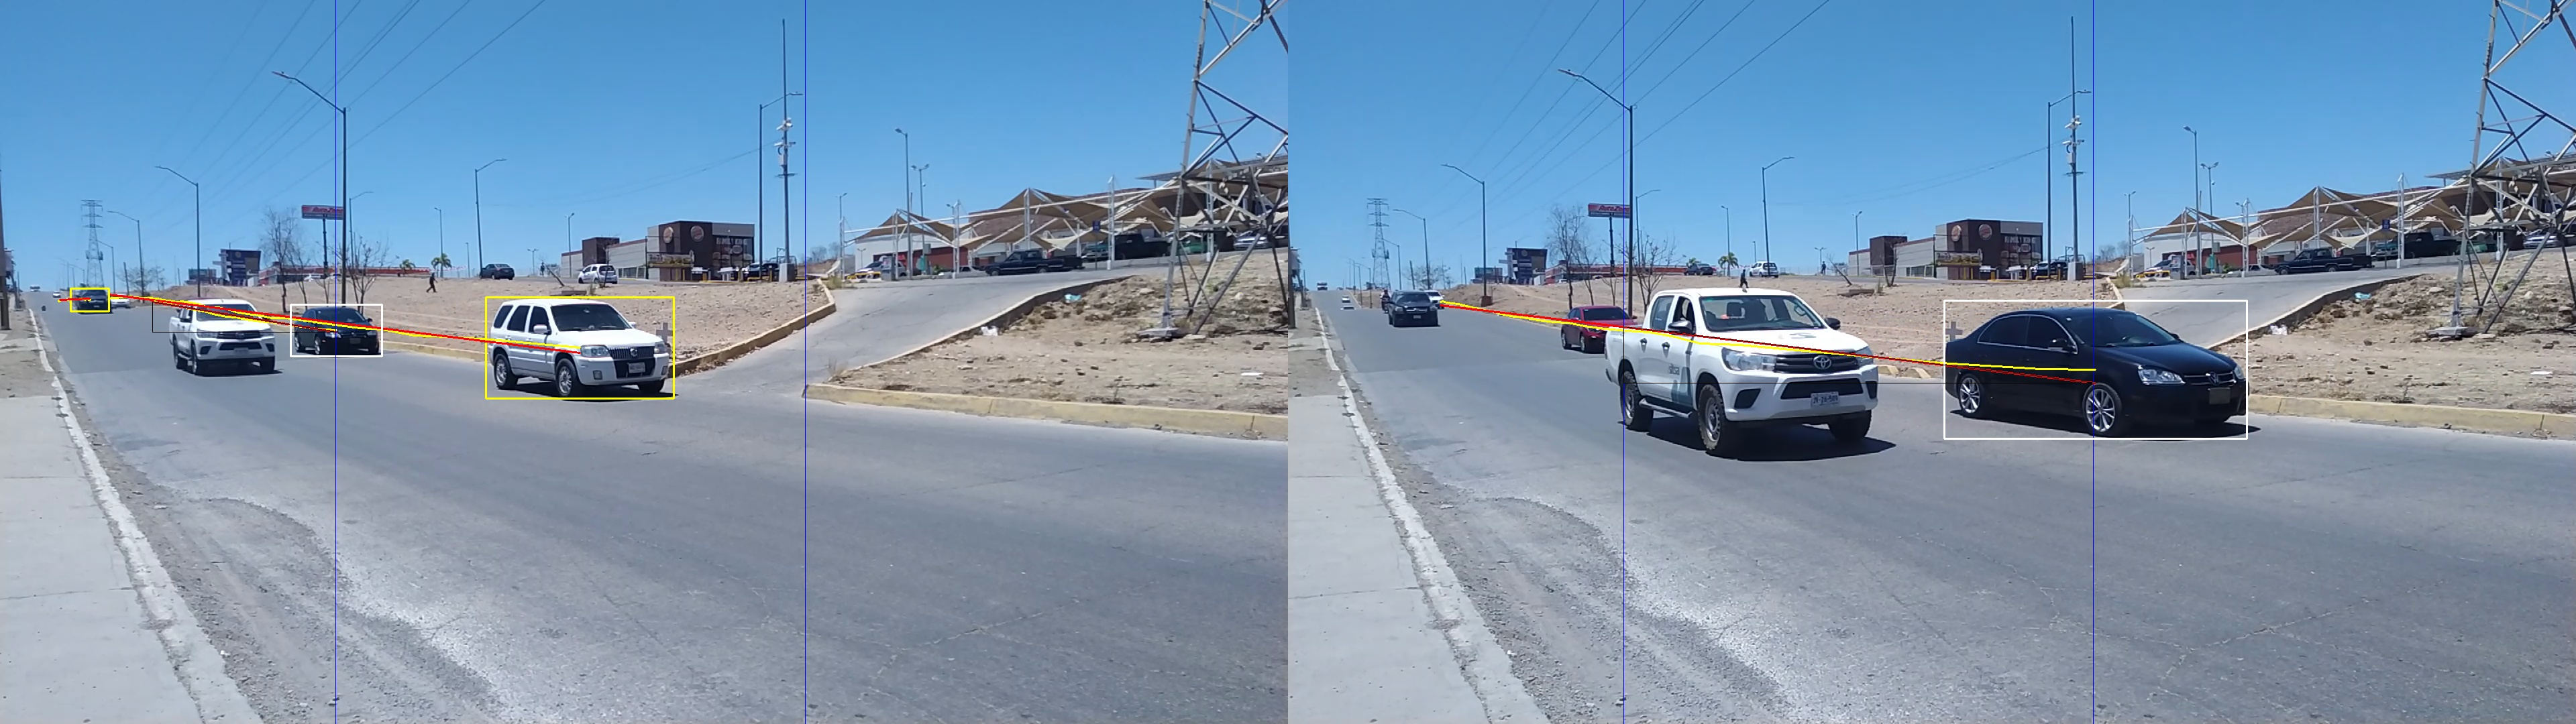
\includegraphics[width=1\textwidth]{Metodologia/imgs/Completo.jpg}
    \caption{Imagen resultado para cada linea de archivo CSV.}
    \label{fig:Completo}
\end{figure}

%%%%%%%%%%%%%%%%%%%%%%%%%%%%%%%%%%%%%%%%%%%%%%%%%%%%%%%%%%%%%%%%%%%%%%%%%%%%%%%%
%%%%%%%%%%%%%%%%%%%%%%%%%%%%%%%%%%%%%%%%%%%%%%%%%%%%%%%%%%%%%%%%%%%%%%%%%%%%%%%%
%%%%%%%%%%%%%%%%%%%%%%%%%%%%%%%%%%%%%%%%%%%%%%%%%%%%%%%%%%%%%%%%%%%%%%%%%%%%%%%%
%%%%%%%%%%%%%%%%%%%%%%%%%%%%%%%%%%%%%%%%%%%%%%%%%%%%%%%%%%%%%%%%%%%%%%%%%%%%%%%%
%%%%%%%%%%%%%%%%%%%%%%%%%%%%%%%%%%%%%%%%%%%%%%%%%%%%%%%%%%%%%%%%%%%%%%%%%%%%%%%%

\subsection{Validación de la extracción de la información}

Una vez que el sistema genera nuestras imágenes de salida y el archivo CSV resultante debemos validar que el vehículo detectado sea el correcto y que el área de detección del vehículo sea lo más completa posible.

Para el caso de validar que el vehículo sea el correcto debemos ver cada una de las imágenes generadas y leer la descripción en el archivo CSV de entrada, en caso de identificar un vehículo que no corresponda debemos modificar los segundos en el archivo CSV de entrada de tal manera que el sistema detecte el correcto, existen dos casos en los que el sistema no podrá identificar el vehículo, que el vehículo correcto sea tapado por otro o que al vehículo no se le haya podido generar su seguimiento completo del punto A al B de forma correcta, para estos caso debemos eliminar la línea correspondiente en el archivo de entrada, para ambos casos ya sea que se tenga que modificar los segundos o se tenga que eliminar la línea debemos ejecutar el sistema nuevamente para que el sistema genere todo de nuevo.

Para validar que el área de detección del vehículo sea lo más completa posible también debemos realizar una inspección visual de las imágenes generadas, en estas podemos identificar cuando un vehículo ha sido detectado completamente, como muestra la Figura \ref{fig:ImagenValida}.

\begin{figure}[H]
    \centering
    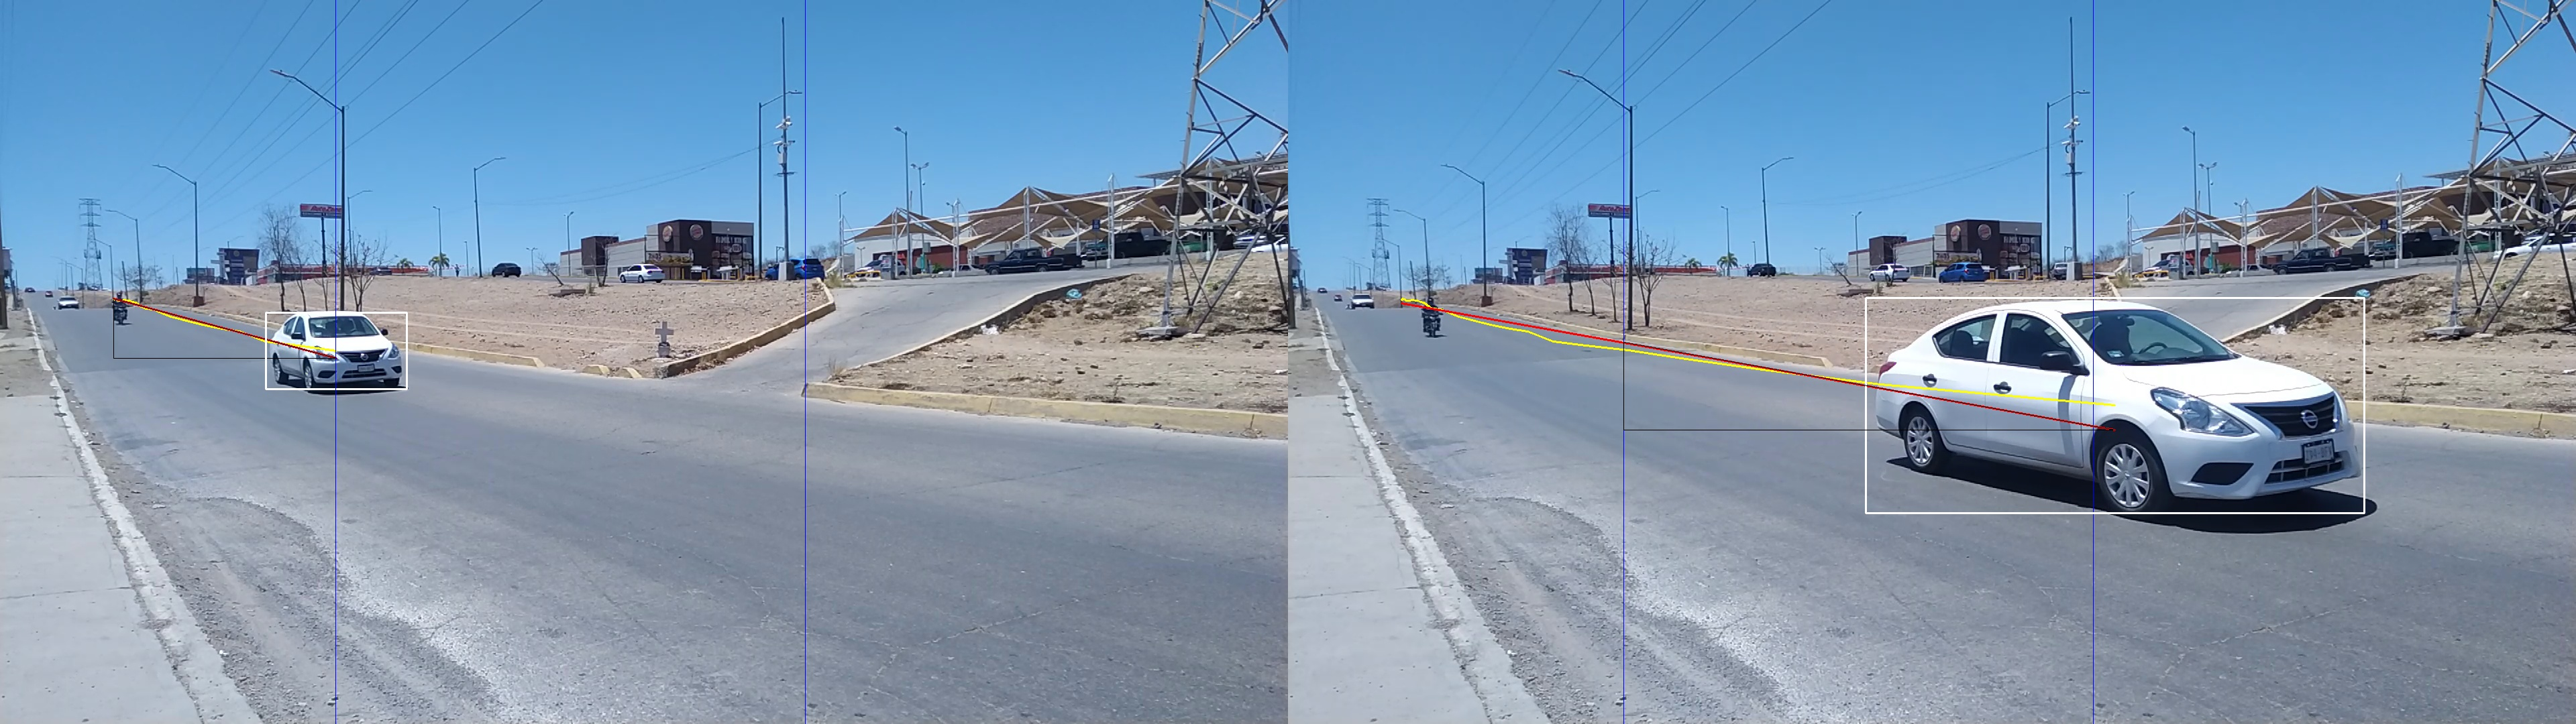
\includegraphics[width=1\textwidth]{Metodologia/imgs/Valido.jpg}
    \caption{Imagen valida representando una linea del archivo CSV.}
    \label{fig:ImagenValida}
\end{figure}

Por otra parte, hay ocasiones en la cuales el sistema solo detecta parte del vehículo, estas imágenes son las que podemos considerar como invalidas, un ejemplo se muestra en la Figura \ref{fig:ImagenInvalida}.

\begin{figure}[H]
    \centering
    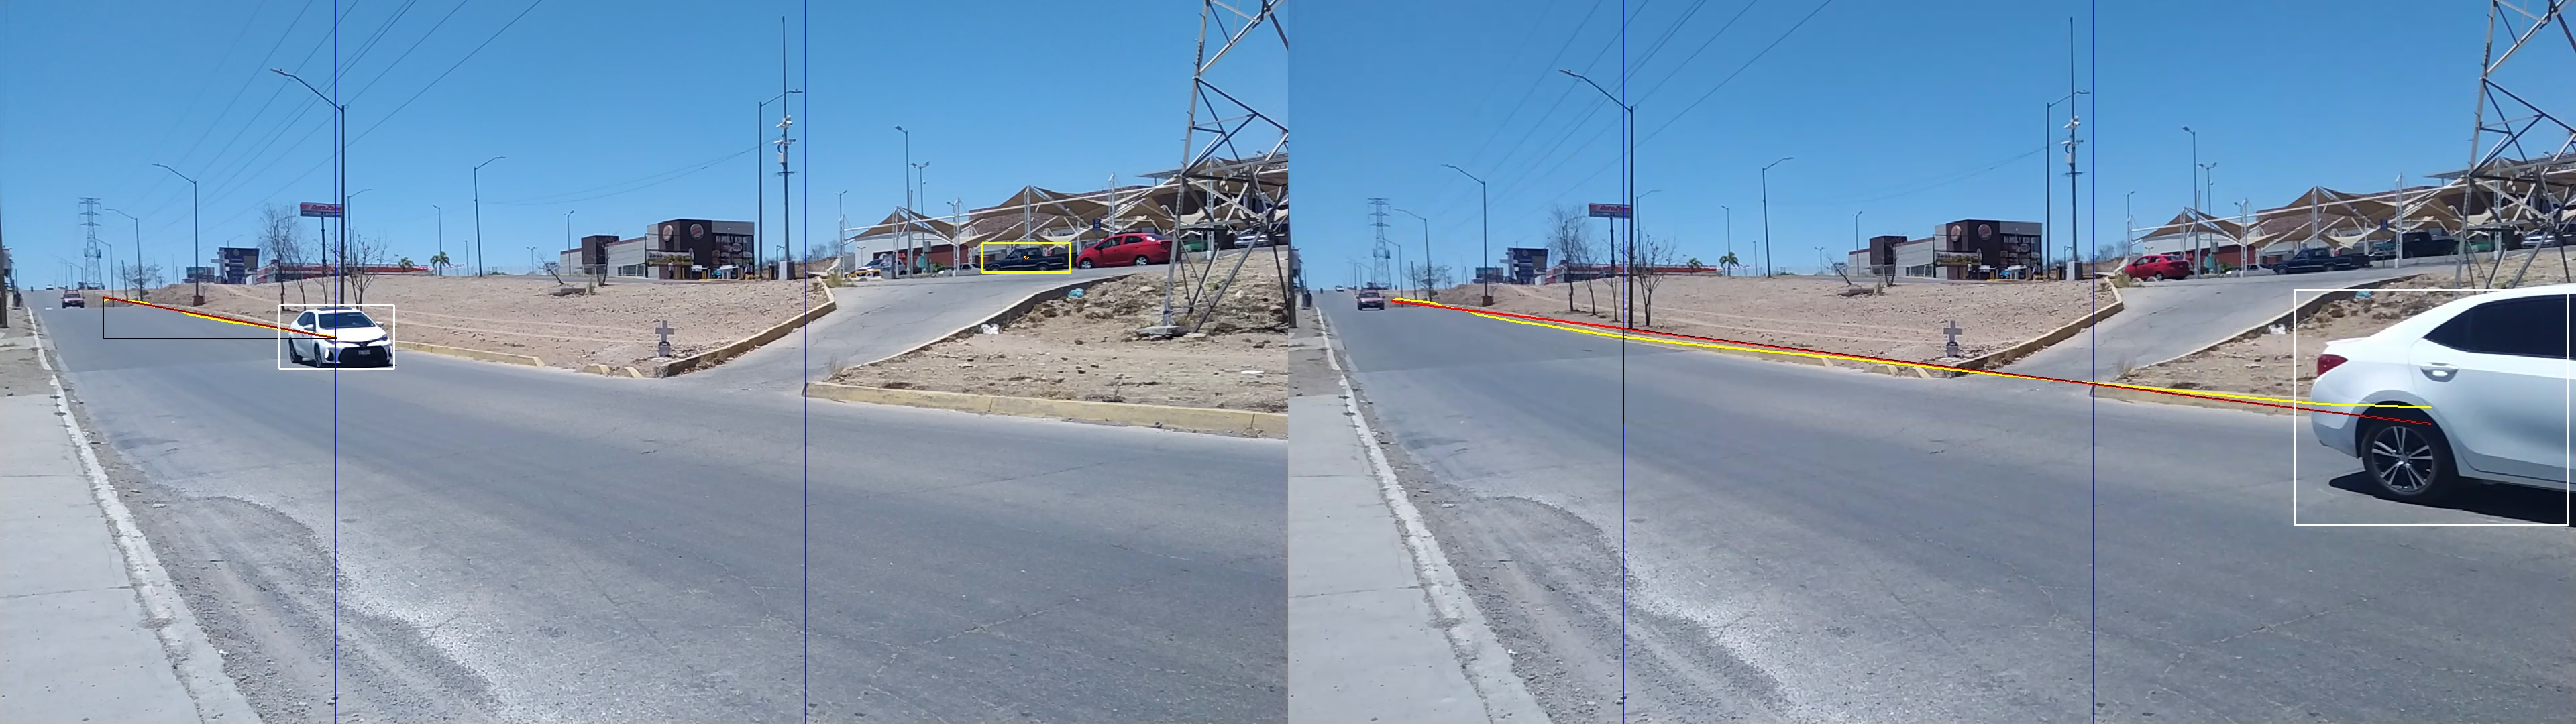
\includegraphics[width=1\textwidth]{Metodologia/imgs/Invalido.jpg}
    \caption{Imagen invalida representando una linea del archivo CSV.}
    \label{fig:ImagenInvalida}
\end{figure}

Una vez que encontramos una imagen invalida procedemos a eliminar la línea correspondiente en el archivo CSV de salida, esta línea la podemos identificar por el identificador del final ya que este corresponde a la imagen. Para este caso no es necesario volver a ejecutar el sistema, pero se recomienda hacer un respaldo del archivo CSV original.
